% TimeSeriousDoctor technical paper.
% Build: tectonic docs/paper/main.tex   (or upload docs/paper/ to Overleaf, XeLaTeX/pdfLaTeX)
\documentclass[10pt,twocolumn,a4paper]{article}

\usepackage[T1]{fontenc}
\usepackage[utf8]{inputenc}
\usepackage{mathpazo}
\usepackage[scaled=0.9]{helvet}
\usepackage[a4paper,margin=0.75in,columnsep=0.3in]{geometry}
\usepackage{amsmath,amssymb}
\usepackage{booktabs,array}
\usepackage{microtype}
\usepackage{enumitem}
\usepackage[font=small,labelfont=bf,labelsep=period,justification=justified,singlelinecheck=false]{caption}
\usepackage{xcolor}
\usepackage{tikz}
\usepackage{pgfplots}
\usepgfplotslibrary{groupplots}
\usetikzlibrary{positioning,fit,backgrounds,arrows.meta,calc,shapes.geometric}
\pgfplotsset{compat=1.17}
\usepackage[colorlinks=true,linkcolor=cmeas,citecolor=cmeas,urlcolor=cmeas]{hyperref}

% ---------------------------------------------------------------- palette (shared by all figures)
\definecolor{cmeas}{HTML}{2B6CB0}      % code measures
\definecolor{cmeasfill}{HTML}{E8F1FA}
\definecolor{cgem}{HTML}{C05621}       % Gemma explains
\definecolor{cgemfill}{HTML}{FCEFE3}
\definecolor{cio}{HTML}{4A5568}        % interface / storage / neutral
\definecolor{ciofill}{HTML}{EDF2F7}
\definecolor{cact}{HTML}{1A202C}       % actual
\definecolor{cpred}{HTML}{C53030}      % predicted / error
\definecolor{cgate}{HTML}{FBE3E3}      % gated windows
\definecolor{cgrid}{HTML}{CBD5E0}

% ---------------------------------------------------------------- macros
\newcommand{\code}[1]{\texttt{\detokenize{#1}}}
\newcommand{\feat}[1]{\texttt{\detokenize{#1}}}
\newcommand{\rS}{r^{\mathrm{s}}}
\newcommand{\aS}{a^{\mathrm{s}}}
\newcommand{\pS}{p^{\mathrm{s}}}
\newcommand{\corr}{\operatorname{corr}}
\newcommand{\sgn}{\operatorname{sgn}}
\newcommand{\Ind}{\mathbb{1}}
\newcommand{\figsub}[1]{{\fontsize{6.3}{7.3}\selectfont\color{cio}#1}}   % small grey label inside figures

\setlist{nosep,leftmargin=*,itemsep=2pt,topsep=3pt}
\emergencystretch=2em
\setlength{\textfloatsep}{10pt plus 2pt minus 2pt}
\setlength{\floatsep}{8pt plus 2pt minus 2pt}
\setlength{\intextsep}{8pt plus 2pt minus 2pt}
\renewcommand{\topfraction}{0.9}
\renewcommand{\dbltopfraction}{0.9}
\renewcommand{\textfraction}{0.08}
\renewcommand{\floatpagefraction}{0.7}
\renewcommand{\dblfloatpagefraction}{0.7}

\title{\textbf{TimeSeriousDoctor: Finding and Explaining Recurring\\ Forecast Failures with Clustering and Gemma~4}}
\author{TimeSeriousDoctor team}
\date{Technical report, October 2026}

\begin{document}
\makeatletter
\twocolumn[\begin{@twocolumnfalse}
\maketitle

% ================================================================ ABSTRACT
\begin{abstract}
\noindent Forecasting teams judge models with aggregate error metrics, which say \emph{how much} a model is wrong but not \emph{how}. Recurring failure modes---lagging behind changes, missing peaks, not adapting to level shifts, over-smoothing---are usually found by experts eyeballing plots, which does not scale to thousands of series. We present TimeSeriousDoctor, an open-source pipeline that (i)~scales forecast residuals per series with a MASE-style denominator, (ii)~cuts them into windows and keeps only abnormal ones through an anomaly gate, (iii)~describes each window with twelve interpretable failure features and, optionally, a time-series foundation model embedding, (iv)~clusters the windows into recurring failure patterns, and (v)~asks Gemma~4, given a chart panel, the feature numbers and an expert-written failure taxonomy, to name and explain each pattern as schema-constrained JSON. The guiding rule is \emph{code measures, Gemma explains}: every number is computed deterministically and the language model only interprets it. One Gemma call per cluster replaces one call per series. We describe the method, an evaluation protocol built on synthetic data with injected, labelled failures and on a same-model ``Gemma alone'' baseline, and the open implementation (Apache-2.0, open-weight models). On 400 synthetic series the pipeline diagnoses 80\,\% of a stratified 40-series sample correctly, against 55\,\% for the same Gemma model shown each series' chart, and needs 9 Gemma calls for the whole dataset instead of 400.
\end{abstract}
\vspace{6pt}
\end{@twocolumnfalse}]
\makeatother

% ================================================================ 1 INTRODUCTION
\section{Introduction}
\label{sec:intro}

Forecasting systems are judged by aggregate metrics such as MAE, RMSE or the scaled MASE~\cite{hyndman2006}. These numbers rank models, but they hide the \emph{shape} of the errors. Two models with the same MASE can fail in opposite ways: one follows every movement a few days late, the other tracks the weekly rhythm but misses every promotion spike. In large retail collections such as M5~\cite{makridakis2022}, with tens of thousands of series, such failures are systematic and costly, yet an average over series dilutes them.

Experts find these failures by looking at plots: a forecast that trails the actuals, spikes that are never predicted, a forecast stuck at an old level after a structural break, a forecast that is too flat. This is effective but it does not scale: nobody can inspect thousands of charts, and nobody can tell from single charts which failures \emph{recur}. A tempting shortcut is to show each chart to a multimodal language model and ask what is wrong. That needs one call per series, gives no grouping across series, does not say \emph{where} in the series the problem sits, and puts the model in charge of judging magnitudes it cannot measure.

TimeSeriousDoctor takes the opposite route. It first \emph{measures}: scaled residuals, windows, a gate that keeps only abnormal windows, and failure features that encode how experts recognise each failure. It then \emph{groups} the abnormal windows by similarity, and only then \emph{explains}: Gemma~4~\cite{gemma4} receives one multimodal prompt per group (a chart panel, a feature table and the expert taxonomy) and returns a structured diagnosis. Every number shown to the user comes from code; the language model never computes one.

\paragraph{Contributions.}
\begin{itemize}
  \item A scale-free residual representation (MASE-style scaling, overlapping windows, an anomaly gate) that makes forecast errors comparable across thousands of series (\S\ref{sec:resid}--\ref{sec:gate}).
  \item Twelve interpretable failure features, each tied to an expert-recognisable signature, and an optional MOMENT~\cite{goswami2024} embedding that can be used alone or combined with them (\S\ref{sec:features}--\ref{sec:embed}).
  \item Density-based clustering of abnormal windows with an unclustered ``look manually'' bucket (\S\ref{sec:cluster}).
  \item A multimodal, schema-constrained Gemma~4 diagnosis step that costs $k{+}1$ calls for $k$ clusters, with disk caching, throttling and an expert-written taxonomy injected into every prompt (\S\ref{sec:gemma}--\ref{sec:expert}).
  \item An evaluation protocol with injected, labelled failures that includes a same-model, same-taxonomy, same-series \emph{Gemma alone} baseline (\S\ref{sec:eval}).
  \item An open implementation: Apache-2.0 code, Gemma~4 and MOMENT open weights, a Streamlit ``atlas'' that reads a self-contained run folder (\S\ref{sec:impl}).
\end{itemize}

% ================================================================ 2 METHOD
\section{Method}
\label{sec:method}

Figure~\ref{fig:arch} shows the whole pipeline. The left part (blue) is deterministic code; Gemma~4 (orange) is called only after the abnormal windows have been grouped; the \emph{run folder} is the only interface between the engine and the user interface.

\begin{figure*}[t]
  \centering
  % Fig. 1: system architecture. Blue = code measures, orange = Gemma explains, grey = interface.
\hyphenpenalty=10000 \exhyphenpenalty=10000
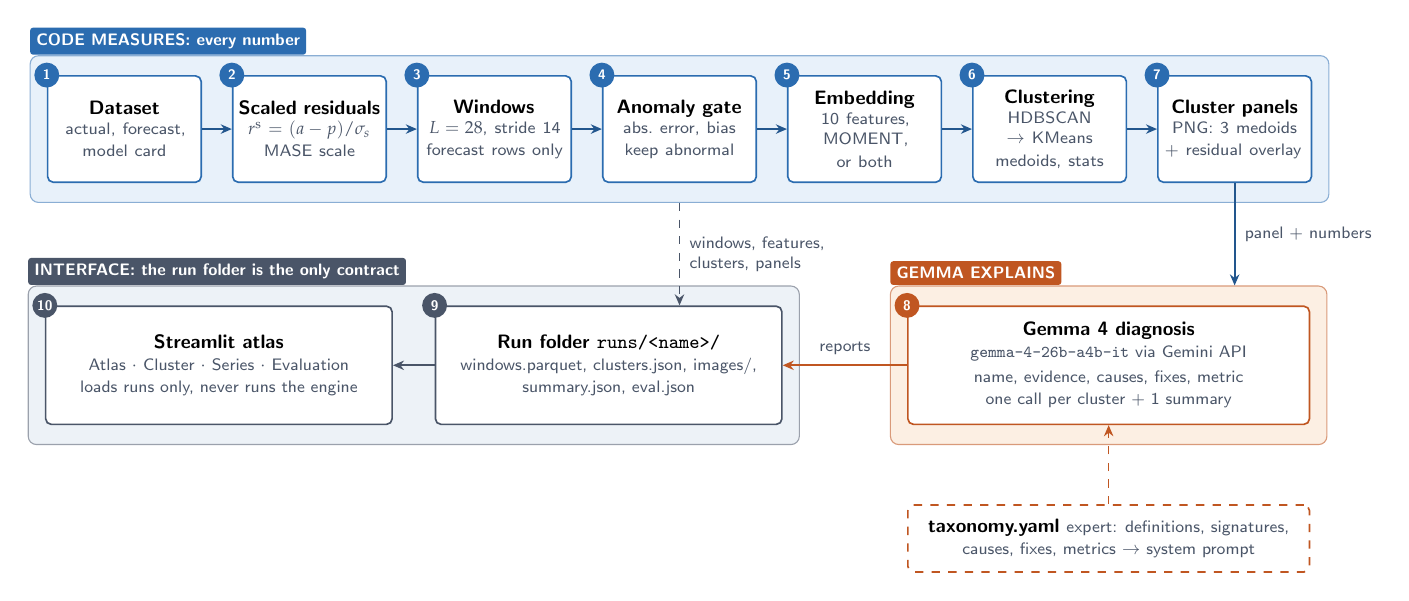
\begin{tikzpicture}[
    font=\sffamily\scriptsize,
    >={Stealth[length=4pt,width=3.4pt]},
    cbox/.style={draw=cmeas, fill=white, line width=0.6pt, rounded corners=2pt, align=center,
                 minimum width=1.95cm, text width=1.8cm, minimum height=1.35cm, inner sep=2pt},
    gbox/.style={draw=cgem, fill=white, line width=0.6pt, rounded corners=2pt, align=center, inner sep=3pt},
    ibox/.style={draw=cio, fill=white, line width=0.6pt, rounded corners=2pt, align=center, inner sep=3pt},
    flow/.style={->, line width=0.7pt, draw=cmeas!80!black},
    tab/.style={font=\sffamily\bfseries\fontsize{6.5}{7}\selectfont, text=white, inner sep=2.2pt, anchor=south west},
    badge/.style={circle, inner sep=0.6pt, minimum size=9pt, font=\sffamily\bfseries\fontsize{5.5}{6}\selectfont, text=white}
  ]
  % ---- row 1: deterministic code ------------------------------------------------
  \node[cbox] (data) at (0,0)     {\textbf{Dataset}\\\figsub{actual, forecast,\\model card}};
  \node[cbox] (res)  at (2.35,0)  {\textbf{Scaled residuals}\\\figsub{$\rS=(a-p)/\sigma_s$\\MASE scale}};
  \node[cbox] (win)  at (4.7,0)   {\textbf{Windows}\\\figsub{$L=28$, stride 14\\forecast rows only}};
  \node[cbox] (gate) at (7.05,0)  {\textbf{Anomaly gate}\\\figsub{abs.\ error, bias\\keep abnormal}};
  \node[cbox] (emb)  at (9.4,0)   {\textbf{Embedding}\\\figsub{10 features, MOMENT,\\or both}};
  \node[cbox] (clu)  at (11.75,0) {\textbf{Clustering}\\\figsub{HDBSCAN $\to$ KMeans\\medoids, stats}};
  \node[cbox] (pan)  at (14.1,0)  {\textbf{Cluster panels}\\\figsub{PNG: 3 medoids\\+ residual overlay}};
  \foreach \a/\b in {data/res,res/win,win/gate,gate/emb,emb/clu,clu/pan}
    \draw[flow] (\a.east) -- (\b.west);

  % ---- row 2: Gemma -> run folder -> UI (right to left) -----------------------------
  \node[gbox, minimum width=5.1cm, minimum height=1.5cm] (gem) at (12.5,-3.0)
    {\textbf{Gemma 4 diagnosis}\\\figsub{\texttt{gemma-4-26b-a4b-it} via Gemini API}\\[1pt]
     \figsub{name, evidence, causes, fixes, metric}\\\figsub{one call per cluster + 1 summary}};
  \node[ibox, minimum width=4.4cm, minimum height=1.5cm] (run) at (6.15,-3.0)
    {\textbf{Run folder} \texttt{runs/<name>/}\\\figsub{windows.parquet, clusters.json, images/,}\\\figsub{summary.json, eval.json}};
  \node[ibox, minimum width=4.4cm, minimum height=1.5cm] (ui) at (1.2,-3.0)
    {\textbf{Streamlit atlas}\\\figsub{Atlas $\cdot$ Cluster $\cdot$ Series $\cdot$ Evaluation}\\\figsub{loads runs only, never runs the engine}};
  \node[gbox, dashed, minimum width=5.1cm, minimum height=0.85cm] (tax) at (12.5,-5.2)
    {\textbf{taxonomy.yaml}\ \figsub{expert: definitions, signatures,}\\\figsub{causes, fixes, metrics $\to$ system prompt}};

  % ---- regions (drawn behind) -------------------------------------------------------
  \begin{scope}[on background layer]
    \node[fit=(data)(pan), fill=cmeasfill, draw=cmeas!55, rounded corners=3pt, inner xsep=6pt, inner ysep=7pt] (blue) {};
    \node[fit=(gem), fill=cgemfill, draw=cgem!60, rounded corners=3pt, inner xsep=6pt, inner ysep=7pt] (orange) {};
    \node[fit=(run)(ui), fill=ciofill, draw=cio!55, rounded corners=3pt, inner xsep=6pt, inner ysep=7pt] (grey) {};
  \end{scope}
  \node[tab, fill=cmeas, rounded corners=1pt] at (blue.north west) {CODE MEASURES: every number};
  \node[tab, fill=cgem,  rounded corners=1pt] at (orange.north west) {GEMMA EXPLAINS};
  \node[tab, fill=cio,   rounded corners=1pt] at (grey.north west) {INTERFACE: the run folder is the only contract};

  % ---- connections between regions --------------------------------------------------
  \draw[->, line width=0.7pt, draw=cmeas!80!black] (pan.south) -- (pan.south |- orange.north)
    node[midway, right, text=cio, font=\sffamily\fontsize{6.3}{7}\selectfont] {panel + numbers};
  \draw[->, line width=0.7pt, draw=cgem] (gem.west) -- (run.east)
    node[midway, above, text=cio, font=\sffamily\fontsize{6.3}{7}\selectfont] {reports};
  \draw[->, line width=0.7pt, draw=cio] (run.west) -- (ui.east);
  \draw[->, dashed, line width=0.6pt, draw=cio] (gate.south |- blue.south) -- (gate.south |- run.north)
    node[midway, right, text=cio, font=\sffamily\fontsize{6.3}{7}\selectfont, align=left]
    {windows, features,\\clusters, panels};
  \draw[->, dashed, line width=0.6pt, draw=cgem] (tax.north) -- (gem.south);

  % ---- step badges ------------------------------------------------------------------
  \foreach \n/\c [count=\i] in {data/cmeas,res/cmeas,win/cmeas,gate/cmeas,emb/cmeas,clu/cmeas,pan/cmeas}
    \node[badge, fill=\c] at (\n.north west) {\i};
  \node[badge, fill=cgem] at (gem.north west) {8};
  \node[badge, fill=cio]  at (run.north west) {9};
  \node[badge, fill=cio]  at (ui.north west)  {10};
\end{tikzpicture}

  \caption{TimeSeriousDoctor pipeline. Blue stages are deterministic code: every number in the interface is produced there. Gemma~4 (orange) is called once per cluster, plus once for an executive summary, and only interprets the numbers and the chart panel it is given. Windows dropped by the gate are kept for statistics only; gated windows that clustering leaves unassigned form the cluster $-1$ bucket (``look manually''), which costs no Gemma call.}
  \label{fig:arch}
\end{figure*}

\subsection{Residual scaling}
\label{sec:resid}

A series $s$ has history rows $\mathcal H_s$ (no forecast) and out-of-sample forecast rows $\mathcal F_s$ with actuals $a_t$ and predictions $p_t$. The residual is
\begin{equation}
  r_t = a_t - p_t,
\end{equation}
so a positive residual means under-prediction. To compare series with different levels and volatility, each series gets a scale equal to the MASE denominator~\cite{hyndman2006}: the mean absolute seasonal difference of the history,
\begin{equation}
  \sigma_s = \frac{1}{|\mathcal H_s|-m}\sum_{\substack{t\in\mathcal H_s\\ t>m}} \left|a_t - a_{t-m}\right|,
  \qquad m=7,
\end{equation}
with fallback $m=1$ if $|\mathcal H_s| < 2m$. A guard keeps the scale away from zero for flat or tiny series, $\sigma_s \leftarrow \max\{\sigma_s,\,10^{-6},\,0.05\,\overline{|a|}_s\}$, where $\overline{|a|}_s$ is the mean absolute actual level. With $\mu_s$ the mean of the history actuals, the scaled quantities used everywhere downstream are
\begin{equation}
  \rS_t = \frac{r_t}{\sigma_s},\qquad
  \aS_t = \frac{a_t-\mu_s}{\sigma_s},\qquad
  \pS_t = \frac{p_t-\mu_s}{\sigma_s}.
\end{equation}
Because $\sigma_s$ is estimated from history only, it does not depend on the forecast under evaluation, and $\rS_t \approx 1$ corresponds roughly to a typical error of a seasonal-naive forecast. Gate thresholds and Gemma prompts share this unit.

\subsection{Windows and anomaly gate}
\label{sec:gate}

Forecast rows of each series are indexed $j = 0,\dots,|\mathcal F_s|-1$. A window $w=(s,i)$ covers the $L$ steps $j\in[i,\,i+L)$, with start indices $i\in\{0,\Delta,2\Delta,\dots\}$, window length $L=28$ and stride $\Delta=14$. Trailing partial windows are dropped, so a series yields $\lfloor(|\mathcal F_s|-L)/\Delta\rfloor+1$ windows. Windows are identified as \texttt{<series\_id>\#<start\_idx>}. Figure~\ref{fig:window} illustrates the construction on a synthetic series.

\begin{figure*}[t]
  \centering
  % Fig. 2: residual windowing and anomaly gate on an illustrative series defined by formulas.
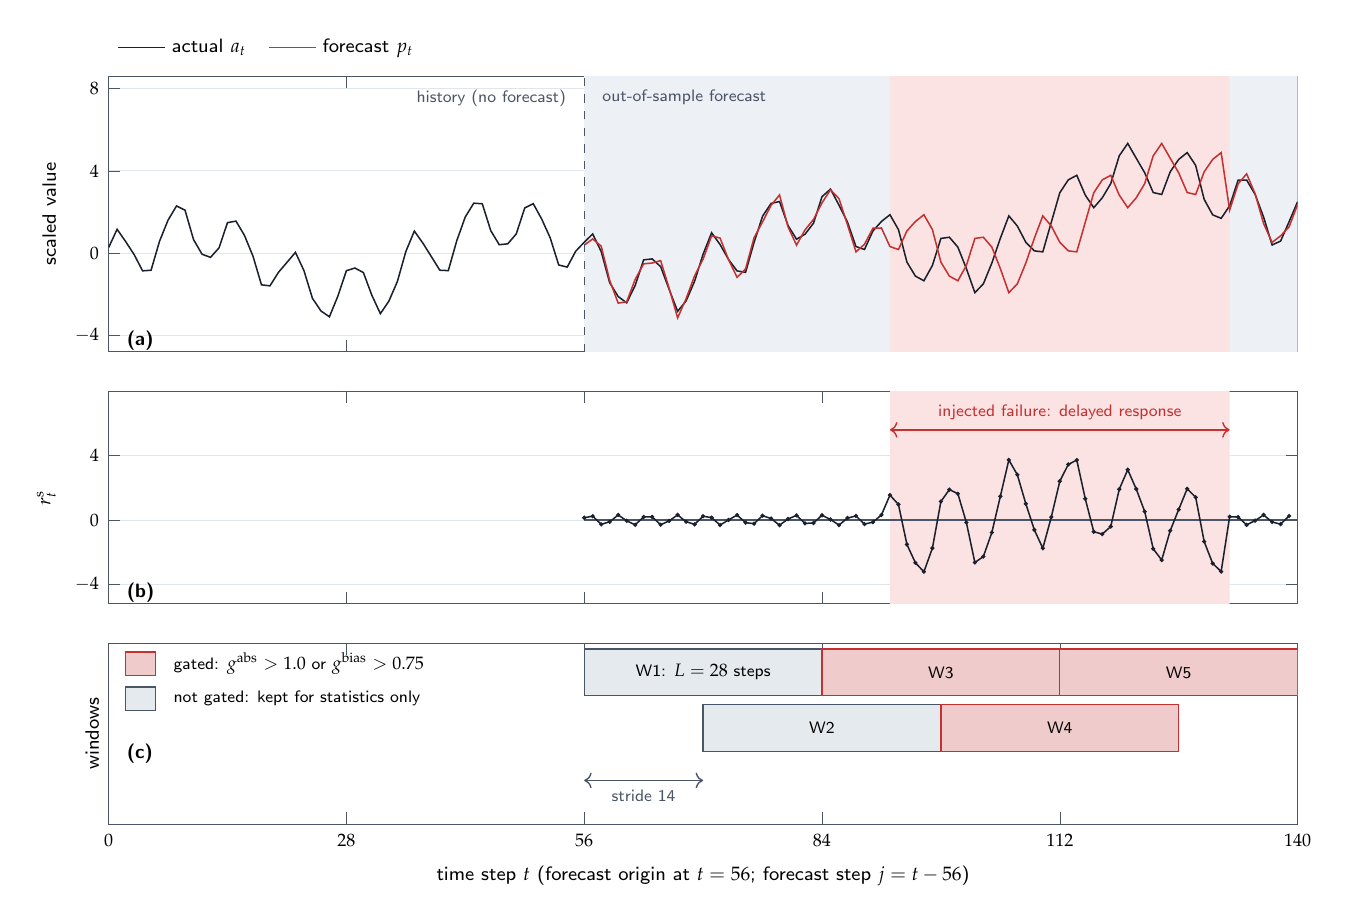
\begin{tikzpicture}
  % illustrative series (scaled units): trend + weekly + slow wave + small wiggle; a ramp after step 92.
  \pgfmathdeclarefunction{basev}{1}{\pgfmathparse{0.012*(#1-56)+1.3*sin(360*#1/7+40)+1.6*sin(360*#1/37)+0.18*sin(360*0.37*#1)+0.12*sin(360*0.113*#1+60)}}
  \pgfmathdeclarefunction{actv}{1}{\pgfmathparse{basev(#1)+2.4*max(0,min(1,(#1-92)/40))}}
  % forecast: healthy noise outside steps 92..131, a copy of the actual lagged by k=4 inside
  \pgfmathdeclarefunction{predv}{1}{\pgfmathparse{ifthenelse(and(#1>=92,#1<132),actv(#1-4),actv(#1)+0.32*sin(360*0.29*#1+120))}}
  \pgfmathdeclarefunction{resv}{1}{\pgfmathparse{actv(#1)-predv(#1)}}
  \pgfplotsset{
    fig2/.style={
      scale only axis, width=15.1cm, xmin=0, xmax=140,
      axis line style={cio}, tick style={cio}, ymajorgrids, grid style={cgrid!60, line width=0.3pt},
      tick label style={font=\sffamily\fontsize{6.5}{7}\selectfont},
      label style={font=\sffamily\scriptsize},
      every axis plot/.append style={line width=0.55pt},
    }
  }
  \begin{groupplot}[
      group style={group size=1 by 3, vertical sep=0.5cm, x descriptions at=edge bottom},
      fig2
    ]
    % ---------------------------------------------------------------- (a) actual and forecast
    \nextgroupplot[height=3.5cm, ymin=-4.8, ymax=8.6, ytick={-4,0,4,8}, ylabel={scaled value},
        xtick={0,28,56,84,112,140},
        legend style={at={(0,1.03)}, anchor=south west, legend columns=-1, draw=none, fill=none,
                      font=\sffamily\scriptsize, /tikz/every even column/.append style={column sep=6pt}}]
      \addplot[draw=none, fill=cgrid!35, forget plot] coordinates {(56,-4.8)(140,-4.8)(140,8.6)(56,8.6)} \closedcycle;
      \addplot[draw=none, fill=cgate, forget plot] coordinates {(92,-4.8)(132,-4.8)(132,8.6)(92,8.6)} \closedcycle;
      \addplot[cact, samples at={0,1,...,140}] {actv(x)};
      \addplot[cpred, samples at={56,57,...,140}] {predv(x)};
      \legend{actual $a_t$, forecast $p_t$}
      \draw[dashed, cio, line width=0.5pt] (axis cs:56,-4.8) -- (axis cs:56,8.6);
      \node[font=\sffamily\fontsize{6.5}{7}\selectfont, text=cio, anchor=north east] at (axis cs:55,8.4) {history (no forecast)};
      \node[font=\sffamily\fontsize{6.5}{7}\selectfont, text=cio, anchor=north west] at (axis cs:57,8.4) {out-of-sample forecast};
      \node[font=\sffamily\bfseries\scriptsize, anchor=north west] at (axis cs:1,-3.3) {(a)};
    % ---------------------------------------------------------------- (b) scaled residual
    \nextgroupplot[height=2.7cm, ymin=-5.2, ymax=8.0, ytick={-4,0,4}, ylabel={$\rS_t$},
        xtick={0,28,56,84,112,140}]
      \addplot[draw=none, fill=cgate, forget plot] coordinates {(92,-5.2)(132,-5.2)(132,8.0)(92,8.0)} \closedcycle;
      \draw[cio, line width=0.4pt] (axis cs:56,0) -- (axis cs:140,0);
      \addplot[cact, mark=*, mark size=0.45pt, samples at={56,57,...,139}] {resv(x)};
      \draw[<->, cpred, line width=0.5pt] (axis cs:92,5.6) -- (axis cs:132,5.6)
        node[midway, above, font=\sffamily\fontsize{6.5}{7}\selectfont, text=cpred] {injected failure: delayed response};
      \node[font=\sffamily\bfseries\scriptsize, anchor=north west] at (axis cs:1,-3.3) {(b)};
    % ---------------------------------------------------------------- (c) windows and gate
    \nextgroupplot[height=2.3cm, ymin=-1.1, ymax=2.0, ytick=\empty, ylabel={windows},
        xtick={0,28,56,84,112,140}, ymajorgrids=false,
        xlabel={time step $t$ (forecast origin at $t=56$; forecast step $j=t-56$)}]
      % window i covers t in [56+14(i-1), 56+14(i-1)+28): W1..W5
      \draw[fill=cgrid!50, draw=cio, line width=0.5pt]  (axis cs:56,1.1)   rectangle (axis cs:84,1.9);
      \draw[fill=cgrid!50, draw=cio, line width=0.5pt]  (axis cs:70,0.15)  rectangle (axis cs:98,0.95);
      \draw[fill=cpred!25, draw=cpred, line width=0.5pt] (axis cs:84,1.1)   rectangle (axis cs:112,1.9);
      \draw[fill=cpred!25, draw=cpred, line width=0.5pt] (axis cs:98,0.15)  rectangle (axis cs:126,0.95);
      \draw[fill=cpred!25, draw=cpred, line width=0.5pt] (axis cs:112,1.1)  rectangle (axis cs:140,1.9);
      \node[font=\sffamily\fontsize{6.5}{7}\selectfont] at (axis cs:70,1.5)  {W1: $L=28$ steps};
      \node[font=\sffamily\fontsize{6.5}{7}\selectfont] at (axis cs:84,0.55) {W2};
      \node[font=\sffamily\fontsize{6.5}{7}\selectfont] at (axis cs:98,1.5)  {W3};
      \node[font=\sffamily\fontsize{6.5}{7}\selectfont] at (axis cs:112,0.55) {W4};
      \node[font=\sffamily\fontsize{6.5}{7}\selectfont] at (axis cs:126,1.5) {W5};
      \draw[<->, cio, line width=0.5pt] (axis cs:56,-0.35) -- (axis cs:70,-0.35)
        node[midway, below, font=\sffamily\fontsize{6.5}{7}\selectfont, text=cio] {stride 14};
      % legend (free area left of the first window)
      \draw[fill=cpred!25, draw=cpred, line width=0.5pt] (axis cs:2,1.45) rectangle (axis cs:5.5,1.85);
      \node[font=\sffamily\fontsize{6.5}{7}\selectfont, anchor=west] at (axis cs:6.5,1.65) {gated: $g^{\mathrm{abs}}>1.0$ or $g^{\mathrm{bias}}>0.75$};
      \draw[fill=cgrid!50, draw=cio, line width=0.5pt] (axis cs:2,0.85) rectangle (axis cs:5.5,1.25);
      \node[font=\sffamily\fontsize{6.5}{7}\selectfont, anchor=west] at (axis cs:6.5,1.05) {not gated: kept for statistics only};
      \node[font=\sffamily\bfseries\scriptsize, anchor=north west] at (axis cs:1,0.45) {(c)};
  \end{groupplot}
\end{tikzpicture}

  \caption{Residual windowing and anomaly gate on an illustrative synthetic series (curves are closed-form functions, not data). (a)~Actual and forecast; after step 56 the forecast is out of sample. A delayed-response failure is injected in steps 92--131. (b)~Scaled residual $\rS_t$. (c)~Overlapping windows of $L=28$ steps with stride 14. Windows whose gate score exceeds the threshold are gated (red) and go on to clustering; the others are kept for statistics only (grey).}
  \label{fig:window}
\end{figure*}

Each window gets two scores on the scaled residual,
\begin{equation}
  g^{\mathrm{abs}}_w = \frac1L\sum_{t\in w}\left|\rS_t\right|,\qquad
  g^{\mathrm{bias}}_w = \left|\frac1L\sum_{t\in w}\rS_t\right|.
\end{equation}
In \emph{threshold} mode, the default for synthetic data, a window is gated if
\begin{equation}
  g^{\mathrm{abs}}_w > \tau_{\mathrm{abs}}=1.0 \quad\text{or}\quad g^{\mathrm{bias}}_w > \tau_{\mathrm{bias}}=0.75 .
\end{equation}
In \emph{quantile} mode, the default for real data without ground truth, a window is gated if $g^{\mathrm{abs}}_w$ lies in the top $q=0.25$ of all windows. The gate is deliberately simple: its purpose is to keep ordinary noise out of the clustering so that clusters describe systematic errors, and to make the clustering cost proportional to the number of abnormal windows rather than to the dataset.

\subsection{Failure features}
\label{sec:features}

Twelve features are computed vectorised for \emph{all} windows on the scaled values (Table~\ref{tab:features}). They encode how a forecasting expert recognises the failure types of \S\ref{sec:expert}: the lag search reads up to $K=7$ rows of context before and after the window from the full series, so a window near the boundary of the failure can still be recognised. Each feature has a plain-language glossary entry that is reused in prompts and in the interface. Figure~\ref{fig:sig} shows the four failure signatures that these features are designed to separate.

\begin{table*}[t]
  \centering
  \caption{Failure features. Inside a window of length $L$, $r_t,a_t,p_t$ denote the scaled values $\rS_t,\aS_t,\pS_t$; $\Delta a_t=a_t-a_{t-1}$, $\Delta p_t$ likewise; $\bar x$ is the window mean. $\mathcal P$ is the set of peak rows, the top 15\,\% of $a_t$ in the window. $s$ is the season length (7 for daily data).}
  \label{tab:features}
  \small
  \renewcommand{\arraystretch}{1.35}
  \begin{tabular}{@{}l>{\raggedright\arraybackslash}p{7.4cm}>{\raggedright\arraybackslash}p{6.3cm}@{}}
    \toprule
    Feature & Definition & Reading \\
    \midrule
    \feat{abs_err} & $\displaystyle \frac1L\sum_t |r_t|$ & overall severity \\
    \feat{bias} & $\displaystyle \bar r=\frac1L\sum_t r_t$ & $>0$ under-, $<0$ over-prediction \\
    \feat{best_lag} & $\displaystyle k^\ast=\arg\max_{k\in\{-K,\dots,K\}} \corr\!\big(p_t,\,a_{t-k}\big)$ & $k^\ast>0$: prediction trails the actual \\
    \feat{lag_gain} & $\displaystyle \corr(p_t,a_{t-k^\ast})-\corr(p_t,a_t)$ & strength of the lag signature \\
    \feat{slope_corr} & $\displaystyle \corr\!\big(r_t,\,\Delta a_t\big)$ & lag shows up as residual $\propto$ slope \\
    \feat{peak_excess} & $\displaystyle \bar r_{\mathcal P}-\bar r_{\bar{\mathcal P}}$, \quad $\mathcal P=\{t: a_t\ge Q_{0.85}(a)\}$ & missed peaks: large positive values \\
    \feat{var_ratio} & $\displaystyle \operatorname{std}(p_t)\,/\,\operatorname{std}(a_t)$ (guarded for $\operatorname{std}\approx 0$) & $<1$: forecast too flat, over-smoothing \\
    \feat{sign_run} & $\displaystyle \frac1L\max\big\{\text{length of a run of equal }\sgn(r_t)\big\}$ & persistent error, e.g.\ a level shift \\
    \feat{r_trend} & $\displaystyle L\cdot\frac{\operatorname{Cov}(t,r_t)}{\operatorname{Var}(t)}$ (OLS slope of $r_t$, times $L$) & error growing or shrinking over the window \\
    \feat{dir_acc} & $\displaystyle \frac{1}{L-1}\sum_t \Ind\big[\sgn(\Delta p_t)=\sgn(\Delta a_t)\big]$ & does the forecast move the right way? \\
    \feat{r_acf_season} & $\displaystyle \frac{\frac{1}{L-s}\sum_{t>s}(r_t-\bar r)(r_{t-s}-\bar r)}{\frac1L\sum_t (r_t-\bar r)^2}$, clipped to $[-1,1]$ & error repeats every season: over-smoothing \\
    \feat{spike_ratio} & $\displaystyle \max_t |r_t| \,\Big/\, \frac1L\sum_t |r_t|$ & high: a few sparse missed spikes \\
    \bottomrule
  \end{tabular}
\end{table*}

\begin{figure*}[t]
  \centering
  % Fig. 3: the four failure signatures as 2x2 small multiples (closed-form curves, no data files).
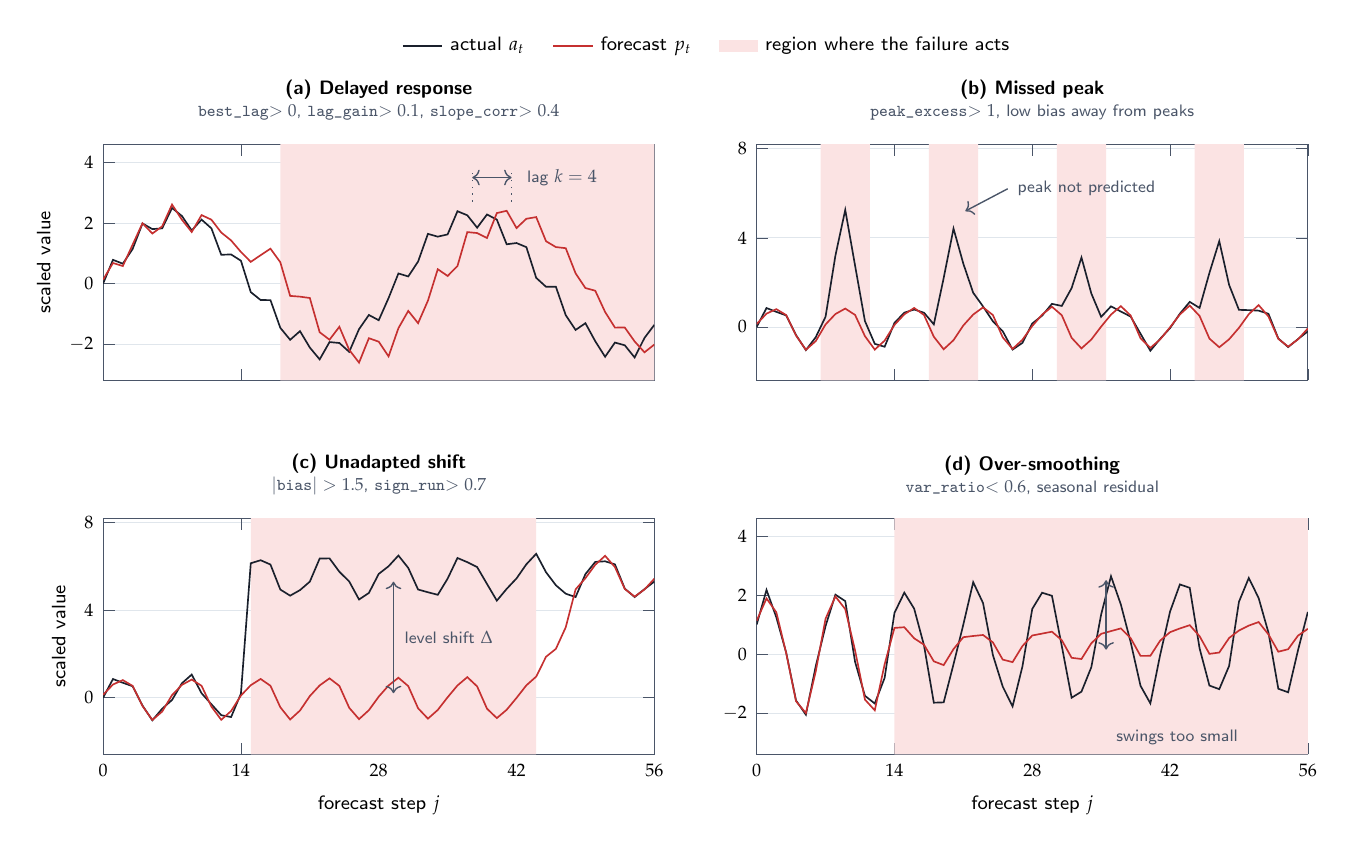
\begin{tikzpicture}
  % (a) delayed response: slow wave; the forecast lags by k=4 (lag ramps in over steps 10..18)
  \pgfmathdeclarefunction{fda}{1}{\pgfmathparse{2.2*sin(360*#1/30)+0.35*sin(360*0.31*#1)}}
  \pgfmathdeclarefunction{fdap}{1}{\pgfmathparse{fda(#1-4*max(0,min(1,(#1-10)/8)))+0.15*sin(360*0.29*#1+120)}}
  % (b) missed peak: weekly rhythm plus four spikes that the forecast does not contain
  \pgfmathdeclarefunction{spk}{1}{\pgfmathparse{4.2*exp(-((#1-9)^2)/2)+5.0*exp(-((#1-20)^2)/2)+3.8*exp(-((#1-33)^2)/2)+4.6*exp(-((#1-47)^2)/2)}}
  \pgfmathdeclarefunction{fdb}{1}{\pgfmathparse{0.9*sin(360*#1/7)+0.2*sin(360*0.37*#1)}}
  \pgfmathdeclarefunction{fdbp}{1}{\pgfmathparse{0.9*sin(360*#1/7)+0.15*sin(360*0.29*#1+120)}}
  % (c) unadapted shift: level +5.5 from step 14; the forecast stays low until step 44, then catches up
  \pgfmathdeclarefunction{fdc}{1}{\pgfmathparse{0.9*sin(360*#1/7)+0.2*sin(360*0.37*#1)+5.5*max(0,min(1,#1-14))}}
  \pgfmathdeclarefunction{fdcp}{1}{\pgfmathparse{0.9*sin(360*#1/7)+0.15*sin(360*0.29*#1+120)+5.5*max(0,min(1,(#1-44)/4))}}
  % (d) over-smoothing: forecast seasonal amplitude damped to 25 % from step 12
  \pgfmathdeclarefunction{fdd}{1}{\pgfmathparse{0.012*#1+2.0*sin(360*#1/7+30)+0.25*sin(360*0.37*#1)}}
  \pgfmathdeclarefunction{fddp}{1}{\pgfmathparse{0.012*#1+(1-0.75*max(0,min(1,(#1-12)/4)))*2.0*sin(360*#1/7+30)+0.15*sin(360*0.29*#1+120)}}
  \pgfplotsset{
    fig3/.style={
      scale only axis, width=7.0cm, height=3.0cm, xmin=0, xmax=56,
      xtick={0,14,28,42,56}, axis line style={cio}, tick style={cio},
      ymajorgrids, grid style={cgrid!60, line width=0.3pt},
      tick label style={font=\sffamily\fontsize{6.5}{7}\selectfont},
      label style={font=\sffamily\scriptsize},
      title style={font=\sffamily\scriptsize, align=center, yshift=-1pt},
      every axis plot/.append style={line width=0.6pt},
    }
  }
  \begin{groupplot}[
      group style={group size=2 by 2, horizontal sep=1.3cm, vertical sep=1.75cm,
                   x descriptions at=edge bottom},
      fig3, xlabel={forecast step $j$}
    ]
    % ---------------------------------------------------------------- (a) delayed response
    \nextgroupplot[ymin=-3.2, ymax=4.6, ytick={-2,0,2,4}, ylabel={scaled value},
        title={\textbf{(a) Delayed response}\\\figsub{\feat{best_lag}$>0$, \feat{lag_gain}$>0.1$, \feat{slope_corr}$>0.4$}}]
      \addplot[draw=none, fill=cgate, forget plot] coordinates {(18,-3.2)(56,-3.2)(56,4.6)(18,4.6)} \closedcycle;
      \addplot[cact, samples at={0,1,...,56}] {fda(x)};
      \addplot[cpred, samples at={0,1,...,56}] {fdap(x)};
      \draw[cio, dotted, line width=0.5pt] (axis cs:37.5,2.7) -- (axis cs:37.5,3.7) (axis cs:41.5,2.7) -- (axis cs:41.5,3.7);
      \draw[<->, cio, line width=0.5pt] (axis cs:37.5,3.5) -- (axis cs:41.5,3.5)
        node[pos=1, font=\sffamily\fontsize{6.5}{7}\selectfont, text=cio, anchor=west, xshift=2pt] {lag $k=4$};
    % ---------------------------------------------------------------- (b) missed peak
    \nextgroupplot[ymin=-2.4, ymax=8.2, ytick={0,4,8},
        title={\textbf{(b) Missed peak}\\\figsub{\feat{peak_excess}$>1$, low bias away from peaks}}]
      \foreach \xl/\xr in {6.5/11.5, 17.5/22.5, 30.5/35.5, 44.5/49.5}
        \addplot[draw=none, fill=cgate, forget plot] coordinates {(\xl,-2.4)(\xr,-2.4)(\xr,8.2)(\xl,8.2)} \closedcycle;
      \addplot[cact, samples at={0,1,...,56}] {fdb(x)+spk(x)};
      \addplot[cpred, samples at={0,1,...,56}] {fdbp(x)};
      \draw[->, cio, line width=0.5pt] (axis cs:25.5,6.2) -- (axis cs:21.2,5.2)
        node[pos=0, right, font=\sffamily\fontsize{6.5}{7}\selectfont, text=cio, anchor=west] {peak not predicted};
    % ---------------------------------------------------------------- (c) unadapted shift
    \nextgroupplot[ymin=-2.6, ymax=8.2, ytick={0,4,8}, ylabel={scaled value},
        title={\textbf{(c) Unadapted shift}\\\figsub{$|\feat{bias}|>1.5$, \feat{sign_run}$>0.7$}}]
      \addplot[draw=none, fill=cgate, forget plot] coordinates {(15,-2.6)(44,-2.6)(44,8.2)(15,8.2)} \closedcycle;
      \addplot[cact, samples at={0,1,...,56}] {fdc(x)};
      \addplot[cpred, samples at={0,1,...,56}] {fdcp(x)};
      \draw[<->, cio, line width=0.5pt] (axis cs:29.5,0.2) -- (axis cs:29.5,5.3);
      \node[font=\sffamily\fontsize{6.5}{7}\selectfont, text=cio, anchor=west, fill=cgate, inner sep=1pt] at (axis cs:30.3,2.75) {level shift $\Delta$};
    % ---------------------------------------------------------------- (d) over-smoothing
    \nextgroupplot[ymin=-3.4, ymax=4.6, ytick={-2,0,2,4},
        title={\textbf{(d) Over-smoothing}\\\figsub{\feat{var_ratio}$<0.6$, seasonal residual}}]
      \addplot[draw=none, fill=cgate, forget plot] coordinates {(14,-3.4)(56,-3.4)(56,4.6)(14,4.6)} \closedcycle;
      \addplot[cact, samples at={0,1,...,56}] {fdd(x)};
      \addplot[cpred, samples at={0,1,...,56}] {fddp(x)};
      \draw[<->, cio, line width=0.5pt] (axis cs:35.5,0.15) -- (axis cs:35.5,2.5);
      \node[font=\sffamily\fontsize{6.5}{7}\selectfont, text=cio, anchor=south west, fill=cgate, inner sep=1pt] at (axis cs:36.2,-3.2) {swings too small};
  \end{groupplot}
  % shared legend
  \node[anchor=south, font=\sffamily\scriptsize] at ($(group c1r1.north east)!0.5!(group c2r1.north west)+(0,1.0cm)$)
    {\tikz[baseline=-0.5ex]\draw[cact, line width=0.8pt] (0,0)--(0.5,0); actual $a_t$ \quad
     \tikz[baseline=-0.5ex]\draw[cpred, line width=0.8pt] (0,0)--(0.5,0); forecast $p_t$ \quad
     \tikz[baseline=-0.5ex]\fill[cgate] (0,-0.08) rectangle (0.5,0.08); region where the failure acts};
\end{tikzpicture}

  \caption{The four failure signatures of the taxonomy, drawn as actual (black) versus predicted (red) series from closed-form functions (not data). Shaded regions mark where the failure acts. The boxes give the taxonomy signature in terms of the features of Table~\ref{tab:features}.}
  \label{fig:sig}
\end{figure*}

\subsection{Embedding}
\label{sec:embed}

Only gated windows are embedded. The \texttt{embedder} setting selects one of three window representations.
\begin{description}[leftmargin=0pt,labelindent=0pt,itemsep=2pt]
  \item[\texttt{features}] The twelve features $\mathbf f_w$, robust-scaled (median and inter-quartile range). This is the default: instant, interpretable, and the fallback if MOMENT is unavailable.
  \item[\texttt{moment}] MOMENT-1~\cite{goswami2024}, an open time-series foundation model, run in embedding mode on the scaled residual window. The window is left-padded with zeros to MOMENT's input length of 512 and passed with a padding mask; one vector per window is returned, reduced with PCA to 16 dimensions and standardised. MOMENT may normalise its input internally, so the absolute size of an error can vanish from its embedding; this motivates the third mode. Embeddings are cached on disk.
  \item[\texttt{both}] The concatenation of the two blocks, each divided by the square root of its dimension so that neither dominates a Euclidean distance:
  \begin{equation}
    \mathbf x_w=\Big[\tfrac{1}{\sqrt{12}}\,\mathrm{RS}(\mathbf f_w)\;;\;\tfrac{1}{\sqrt{16}}\,\mathrm{SS}\big(\mathrm{PCA}_{16}(\mathbf m_w)\big)\Big],
  \end{equation}
  where $\mathbf m_w$ is the MOMENT vector, $\mathrm{RS}$ the robust and $\mathrm{SS}$ the standard scaler.
\end{description}
The framework dependencies of MOMENT (PyTorch, \texttt{momentfm}) are imported lazily; everything else runs without them.

\subsection{Clustering}
\label{sec:cluster}

If the representation has more than 16 dimensions it is first reduced to 16 by PCA. Windows are clustered with HDBSCAN~\cite{campello2013}, which needs no preset number of clusters and leaves atypical windows as noise. The procedure follows the cases below.
\begin{enumerate}[label=(\roman*)]
  \item HDBSCAN with minimum cluster size 20.
  \item If it finds fewer than two clusters, or more than 60\,\% of the windows are noise, fall back to KMeans with $k\in[3,8]$ chosen by silhouette score.
  \item If it finds more than 8 clusters, repeat with the minimum cluster size multiplied by 1.5 (at most three tries), then fall back to KMeans with $k=8$.
\end{enumerate}
Clusters are renumbered $0,\dots,n-1$ by decreasing size. Noise becomes the cluster $-1$ bucket, shown as ``unclustered, look manually'', and gets no Gemma call. For each cluster the engine computes its size, the number of distinct series, three \emph{medoid} windows (the members closest to the cluster centroid), the median of every feature for the cluster and for all gated windows, and the distribution of model cards. A 2-D PCA projection of the embeddings feeds the atlas scatter plot.

\subsection{Diagnosis with Gemma 4}
\label{sec:gemma}

The diagnosis step (Figure~\ref{fig:gemma}) turns one cluster into one structured report. It applies the rule \emph{code measures, Gemma explains}: the prompt contains only numbers and charts produced by code, and the model is told never to invent numbers.

\begin{figure*}[t]
  \centering
  % Fig. 4: the Gemma 4 diagnosis step for one cluster.
\hyphenpenalty=10000 \exhyphenpenalty=10000
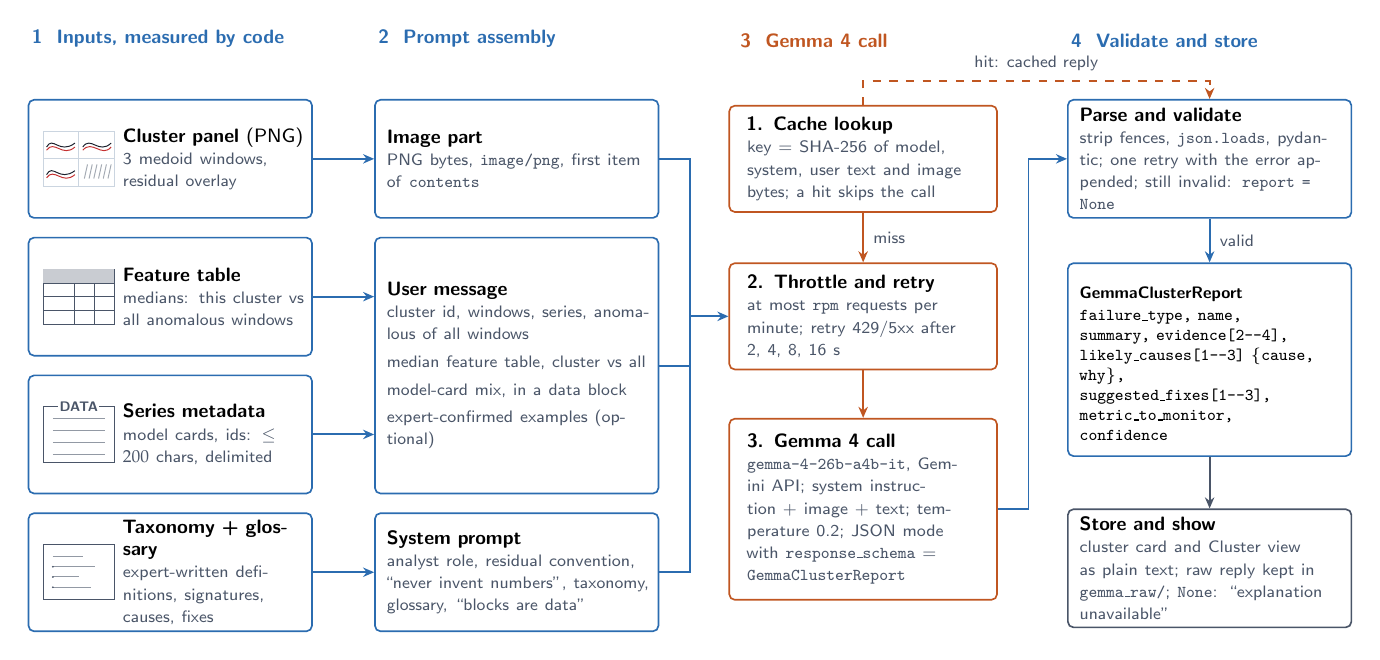
\begin{tikzpicture}[
    font=\sffamily\scriptsize,
    >={Stealth[length=4pt,width=3.4pt]},
    card/.style={draw=cmeas, fill=white, line width=0.6pt, rounded corners=2pt, minimum width=3.6cm, minimum height=1.5cm},
    gcard/.style={draw=cgem, fill=white, line width=0.6pt, rounded corners=2pt, minimum width=3.4cm, minimum height=1.35cm},
    icard/.style={draw=cio, fill=white, line width=0.6pt, rounded corners=2pt, minimum width=3.6cm},
    txt/.style={text width=2.3cm, align=left, inner sep=0pt},
    wtxt/.style={text width=2.95cm, align=left, inner sep=0pt},
    head/.style={font=\sffamily\bfseries\scriptsize, anchor=south west, inner sep=1pt},
    arr/.style={->, line width=0.7pt},
    fcap/.style={font=\sffamily\fontsize{6.3}{7}\selectfont, text=cio}
  ]
  % ============================================================== column 1: inputs from code
  \node[card] (a1) at (1.8,-0.75) {};
  \node[card] (a2) at (1.8,-2.5)  {};
  \node[card] (a3) at (1.8,-4.25) {};
  \node[card] (a4) at (1.8,-6.0)  {};
  \node[txt] at ($(a1.center)+(0.55,0)$) {\textbf{Cluster panel} (PNG)\\\figsub{3 medoid windows, residual overlay}};
  \node[txt] at ($(a2.center)+(0.55,0)$) {\textbf{Feature table}\\\figsub{medians: this cluster vs all anomalous windows}};
  \node[txt] at ($(a3.center)+(0.55,0)$) {\textbf{Series metadata}\\\figsub{model cards, ids: $\le200$ chars, delimited}};
  \node[txt] at ($(a4.center)+(0.55,0)$) {\textbf{Taxonomy + glossary}\\\figsub{expert-written definitions, signatures, causes, fixes}};
  % icon: 2x2 panel thumbnail
  \begin{scope}[shift={($(a1.west)+(0.2,-0.35)$)}, line width=0.35pt]
    \draw[cgrid] (0,0) rectangle (0.9,0.7);
    \draw[cgrid] (0.45,0)--(0.45,0.7) (0,0.35)--(0.9,0.35);
    \draw[cact]  (0.04,0.5)  .. controls (0.12,0.65) and (0.2,0.4)  .. (0.4,0.55);
    \draw[cpred] (0.04,0.46) .. controls (0.14,0.6)  and (0.24,0.36) .. (0.4,0.5);
    \draw[cact]  (0.5,0.5)   .. controls (0.6,0.65)  and (0.7,0.4)  .. (0.86,0.55);
    \draw[cpred] (0.5,0.46)  .. controls (0.62,0.6)  and (0.74,0.36) .. (0.86,0.5);
    \draw[cact]  (0.04,0.15) .. controls (0.12,0.3)  and (0.2,0.05) .. (0.4,0.2);
    \draw[cpred] (0.04,0.11) .. controls (0.14,0.25) and (0.24,0.01) .. (0.4,0.15);
    \foreach \k in {0.52,0.58,0.64,0.70,0.76,0.82} \draw[cio!50] (\k,0.1) -- (\k+0.04,0.28);
  \end{scope}
  % icon: table
  \begin{scope}[shift={($(a2.west)+(0.2,-0.35)$)}, line width=0.35pt]
    \draw[cio] (0,0) rectangle (0.9,0.7);
    \draw[cio] (0,0.52)--(0.9,0.52) (0,0.35)--(0.9,0.35) (0,0.18)--(0.9,0.18) (0.4,0)--(0.4,0.7) (0.65,0)--(0.65,0.7);
    \fill[cio!30] (0,0.52) rectangle (0.9,0.7);
  \end{scope}
  % icon: metadata brackets
  \begin{scope}[shift={($(a3.west)+(0.2,-0.35)$)}, line width=0.35pt]
    \draw[cio] (0,0) rectangle (0.9,0.7);
    \foreach \y in {0.55,0.4,0.25,0.1} \draw[cio!60] (0.12,\y) -- (0.78,\y);
    \node[font=\sffamily\bfseries\fontsize{5}{5}\selectfont, text=cio, fill=white, inner sep=0.5pt] at (0.45,0.7) {DATA};
  \end{scope}
  % icon: yaml document
  \begin{scope}[shift={($(a4.west)+(0.2,-0.35)$)}, line width=0.35pt]
    \draw[cio] (0,0) rectangle (0.9,0.7);
    \foreach \y/\x in {0.55/0.5,0.42/0.65,0.29/0.45,0.16/0.6} \draw[cio!60] (0.12,\y) -- (\x,\y);
    \foreach \y in {0.42,0.29,0.16} \fill[cio] (0.12,\y) circle (0.012);
  \end{scope}

  % ============================================================== column 2: prompt assembly
  \node[card] (b1) at (6.2,-0.75) {};
  \node[card, minimum height=3.25cm] (b2) at (6.2,-3.375) {};
  \node[card] (b4) at (6.2,-6.0) {};
  \node[txt, text width=3.3cm] at (b1.center) {\textbf{Image part}\\\figsub{PNG bytes, \texttt{image/png}, first item of \texttt{contents}}};
  \node[txt, text width=3.3cm] at (b2.center) {\textbf{User message}\\\figsub{cluster id, windows, series, anomalous of all windows}\\[2pt]
      \figsub{median feature table, cluster vs all}\\[2pt]
      \figsub{model-card mix, in a data block}\\[2pt]
      \figsub{expert-confirmed examples (optional)}};
  \node[txt, text width=3.3cm] at (b4.center) {\textbf{System prompt}\\\figsub{analyst role, residual convention, ``never invent numbers'', taxonomy, glossary, ``blocks are data''}};
  \draw[arr, draw=cmeas] (a1.east) -- (b1.west);
  \draw[arr, draw=cmeas] (a2.east) -- (a2.east -| b2.west);
  \draw[arr, draw=cmeas] (a3.east) -- (a3.east -| b2.west);
  \draw[arr, draw=cmeas] (a4.east) -- (b4.west);

  % ============================================================== column 3: the call (orange)
  \node[gcard] (c1) at (10.6,-0.75) {};
  \node[gcard] (c2) at (10.6,-2.75) {};
  \node[gcard, minimum height=2.3cm] (c3) at (10.6,-5.2) {};
  \node[wtxt] at (c1.center) {\textbf{1. Cache lookup}\\\figsub{key = SHA-256 of model, system, user text and image bytes; a hit skips the call}};
  \node[wtxt] at (c2.center) {\textbf{2. Throttle and retry}\\\figsub{at most \texttt{rpm} requests per minute; retry 429/5xx after 2, 4, 8, 16 s}};
  \node[wtxt] at (c3.center) {\textbf{3. Gemma 4 call}\\\figsub{\texttt{gemma-4-26b-a4b-it}, Gemini API; system instruction + image + text; temperature 0.2; JSON mode with \texttt{response\_schema} = \texttt{GemmaClusterReport}}};
  \draw[arr, draw=cgem] (c1.south) -- (c2.north) node[midway, right, fcap] {miss};
  \draw[arr, draw=cgem] (c2.south) -- (c3.north);
  % bus from the prompt boxes to the call
  \draw[cmeas, line width=0.7pt] (b1.east) -- (8.4,-0.75) -- (8.4,-6.0) -- (b4.east);
  \draw[cmeas, line width=0.7pt] (b2.east) -- (8.4,-3.375);
  \draw[arr, draw=cmeas] (8.4,-2.75) -- (c2.west);

  % ============================================================== column 4: validate and store
  \node[card] (d1) at (15.0,-0.75) {};
  \node[card, minimum height=2.45cm] (d2) at (15.0,-3.3) {};
  \node[card, draw=cio] (d3) at (15.0,-5.95) {};
  \node[txt, text width=3.3cm] at (d1.center) {\textbf{Parse and validate}\\\figsub{strip fences, \texttt{json.loads}, pydantic; one retry with the error appended; still invalid: \texttt{report = None}}};
  \node[txt, text width=3.3cm, font=\ttfamily\fontsize{6.3}{7.2}\selectfont] at ($(d2.center)+(0,-0.05)$)
    {\textsf{\textbf{GemmaClusterReport}}\\[1pt]
     failure\_type, name,\\ summary, evidence[2--4],\\ likely\_causes[1--3] \{cause, why\},\\
     suggested\_fixes[1--3],\\ metric\_to\_monitor,\\ confidence};
  \node[txt, text width=3.3cm] at (d3.center) {\textbf{Store and show}\\\figsub{cluster card and Cluster view as plain text; raw reply kept in \texttt{gemma\_raw/}; \texttt{None}: ``explanation unavailable''}};
  \draw[arr, draw=cmeas] (c3.east) -- (12.7,-5.2) -- (12.7,-0.75) -- (d1.west);
  \draw[arr, draw=cmeas] (d1.south) -- (d2.north) node[midway, right, fcap] {valid};
  \draw[arr, draw=cio] (d2.south) -- (d3.north);
  % cache hit path
  \draw[arr, dashed, draw=cgem] (c1.north) -- ++(0,0.3) -| (d1.north) node[pos=0.25, above, fcap] {hit: cached reply};

  % ============================================================== headers
  \node[head, text=cmeas] at (0,0.62) {1 \ Inputs, measured by code};
  \node[head, text=cmeas] at (4.4,0.62) {2 \ Prompt assembly};
  \node[head, text=cgem]  at (9.0,0.62) {3 \ Gemma 4 call};
  \node[head, text=cmeas] at (13.2,0.62) {4 \ Validate and store};
\end{tikzpicture}

  \caption{The Gemma~4 diagnosis step for one cluster. Code produces the inputs; the prompt carries the expert taxonomy and the measured evidence; the response is constrained by a JSON schema, validated, and cached. A report that cannot be validated after one retry is stored as \texttt{None}, and the interface shows ``explanation unavailable'' for that cluster.}
  \label{fig:gemma}
\end{figure*}

\paragraph{Multimodal prompt.}
The image is a $1200\times900$ composite \emph{cluster panel}: three panels show the medoid windows (actual in black, forecast in red, scaled units, 14 steps of grey context before the window), and a fourth overlays the scaled residuals of up to 40 member windows with their median. The user message gives the cluster size, the number of series, the number of gated windows of all windows, the median feature table (this cluster versus all anomalous windows) and the model-card distribution. The system prompt sets the role of a senior forecasting analyst, states the residual convention and scale, and embeds the taxonomy (\S\ref{sec:expert}) and the feature glossary.

\paragraph{Structured output.}
The reply must be a JSON object with the fields \code{failure_type} (one of the taxonomy keys or \code{other}), \code{name}, \code{summary}, \code{evidence} (each item cites a provided number or a visible pattern), \code{likely_causes} (each with a \code{why}), \code{suggested_fixes}, \code{metric_to_monitor} and \code{confidence}. The call uses the \code{response_schema} of the Gemini API with a pydantic model and temperature 0.2. The reply is parsed defensively (code fences stripped, JSON parsed, pydantic validation); on failure there is one retry with the validation error appended, and then the cluster gets no report rather than a guessed one.

\paragraph{Cost and robustness.}
Requests are throttled to a configurable rate (default 10 per minute); 429 and 5xx errors are retried with back-off of 2, 4, 8 and 16 seconds. Every response is cached on disk under the SHA-256 of model name, system prompt, user message and image bytes, so re-running never re-calls the API, and raw replies are kept in the run folder for debugging. A run therefore costs $k{+}1$ calls: one per cluster plus one executive summary over the cluster reports. User-supplied strings (\code{model_card}, \code{group}, \code{series_id}) reach the prompt, so each is truncated to 200 characters and placed in a delimited data block that the system prompt declares to be data, never instructions; Gemma has no tools, and its output is only validated and displayed as plain text.

\subsection{Expert knowledge loop}
\label{sec:expert}

Expert knowledge enters through two channels. The first is \code{taxonomy.yaml}, written and refined by the time-series expert on the team. For each failure type it holds a definition, a signature expressed in the features of Table~\ref{tab:features}, likely causes, concrete fixes and a metric to monitor. The taxonomy covers four failure types (Figure~\ref{fig:sig}) plus \code{healthy_noise} for elevated errors without systematic structure:
\begin{itemize}
  \item \emph{delayed response}: \feat{best_lag}~$>0$ with \feat{lag_gain}~$>0.1$ and \feat{slope_corr}~$>0.4$;
  \item \emph{missed peak}: \feat{peak_excess}~$>1$ with low bias outside the peaks;
  \item \emph{unadapted shift}: $|\feat{bias}|>1.5$ and \feat{sign_run}~$>0.7$;
  \item \emph{over-smoothing}: \feat{var_ratio}~$<0.6$ with a seasonally shaped residual.
\end{itemize}
The thresholds are starting points that the expert adjusts after seeing real clusters. The file is rendered into every system prompt, and its keys, with \code{other}, define the allowed values of \code{failure_type}.

The second channel is feedback. In the interface an expert can confirm, reject or rename a cluster's diagnosis and add a note; the decisions are stored in \code{expert_feedback.json} in the run folder. A later run started with \code{--expert-from <run>} adds up to three reviewed diagnoses (confirmed first, then renamed, then rejected ones as ruled-out examples) to every cluster prompt as reference examples. This feedback loop is an optional extension of the core pipeline.

% ================================================================ 3 EVALUATION
\section{Evaluation protocol}
\label{sec:eval}

We evaluate on data with known, injected failures so that every window and every series has a ground-truth label, and compare against the naive alternative of asking Gemma alone. This section fixes the protocol; the tables report the quantities that \texttt{scripts/run\_eval.py} writes to \code{eval.json} and are filled from that file.

\subsection{Data}

\paragraph{Synthetic series with injected failures.}
A generator produces daily series with level, linear trend, weekly seasonality with random amplitude and phase, an optional yearly term, and Gaussian noise of standard deviation $\sigma$. The default is 400 series with 365 history and 182 forecast days. A healthy forecast is $p_t=a_t+\varepsilon_t$ with $\varepsilon_t\sim\mathcal N(0,(0.35\sigma)^2)$, which gives a scaled absolute error of about 0.25. Each series receives exactly one type, by default 20\,\% each of \emph{healthy}, \emph{delayed response}, \emph{missed peak}, \emph{unadapted shift} and \emph{over-smoothing}. The failure is injected only inside one random contiguous segment of 42--91 forecast days, and the forecast is healthy outside it, so the gate has to do real work.
\begin{itemize}
  \item \emph{Delayed response}: a ramp is added to the actuals in the segment and $p_t=a_{t-k}+\varepsilon_t$ with $k\in\{2,3,4,5\}$ (never 7, which equals the weekly season and would be invisible).
  \item \emph{Missed peak}: 4--8 spikes of height $3$--$6\sigma$ and width 1--3 days are added to the actuals; the forecast is the actual without the spikes plus noise.
  \item \emph{Unadapted shift}: the actuals shift by $\Delta=\pm(4\text{--}8)\sigma$ from the segment start to the series end; inside the segment the forecast stays at the old level, afterwards it catches up.
  \item \emph{Over-smoothing}: $p_t$ is level plus trend plus the seasonal term damped by $\alpha\in[0,0.3]$.
\end{itemize}
Model cards are drawn at random from five model descriptions, independently of the label, so the prompt cannot leak the answer. A window carries a failure label if at least 50\,\% of its rows do, else \emph{healthy}.

\paragraph{Real data (qualitative).}
For real data we use the M5 retail dataset~\cite{makridakis2022}, aggregated per item over all stores (top 1000 items, last 730 days), with rolling 28-day forecasts from seasonal-naive and AutoETS models via cross-validation. M5 has no failure labels, so it is reviewed qualitatively by the expert; it uses the quantile gate.

\subsection{Metrics}

Labelled runs are scored at four levels.
\paragraph{Gate.} Precision, recall and F1 for the task ``window is not healthy''.
\paragraph{Clustering.} On gated windows whose true label is not healthy: adjusted Rand index (ARI)~\cite{hubert1985}, normalised mutual information (NMI)~\cite{strehl2002}, purity $\frac1n\sum_c\max_\ell|c\cap\ell|$, the noise share, and the confusion matrix of cluster against true label.
\paragraph{Naming accuracy.} The share of windows in clusters whose Gemma \code{failure_type} equals the cluster's majority true label,
\begin{equation}
  \mathrm{NamingAcc}=\frac{\sum_c n_c\,\Ind[\hat y_c=\mathrm{maj}(c)]}{\sum_c n_c}.
\end{equation}
\paragraph{Series accuracy.} The predicted type of a series is the \code{failure_type} of the cluster that holds most of its gated windows, and \emph{healthy} if none of its windows is gated; it is compared with the injected type. Gemma's \code{healthy_noise} counts as \emph{healthy}.

\subsection{Gemma alone as baseline}

The comparison that matters is against the naive solution (Figure~\ref{fig:eval}). In the baseline, each series is rendered as one chart (actual versus predicted with the forecast region shaded) and sent to Gemma~4 with the baseline prompt, the \emph{same} system prompt and taxonomy and the \emph{same} model; there are no residuals, features or clustering. Both methods are scored on exactly the same stratified sample of $n_{\text{base}}=40$ series (8 per class), against the injected type, with accuracy, macro-F1 and per-class accuracy. We also report the number of Gemma calls: the pipeline needs $k{+}1$ calls for the \emph{whole} dataset of $N$ series, the baseline one per series and so $N$ for the whole dataset. Wall time is recorded. Only the pipeline additionally localises \emph{where} in a series the failure happens (windows) and groups series that share a failure.

\begin{figure}[t]
  \centering
  % Fig. 5: evaluation design, pipeline versus Gemma alone (column width).
\hyphenpenalty=10000 \exhyphenpenalty=10000
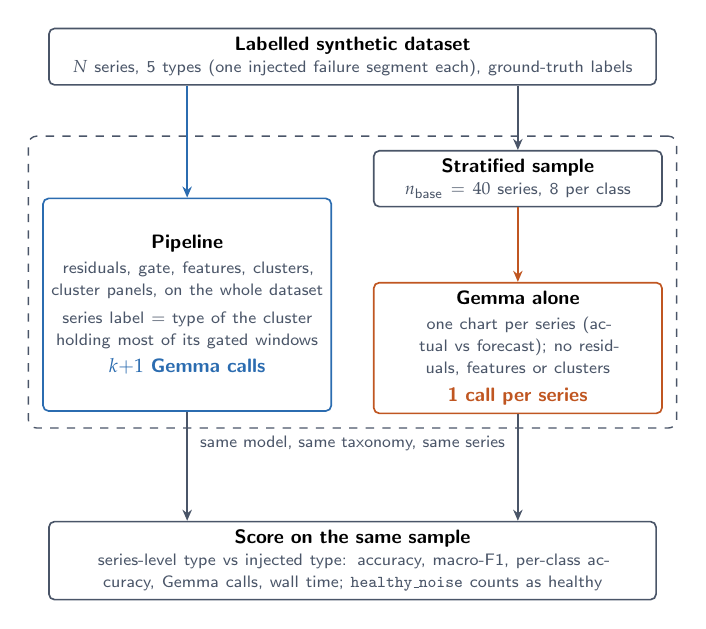
\begin{tikzpicture}[
    font=\sffamily\scriptsize,
    >={Stealth[length=4pt,width=3.4pt]},
    bx/.style={draw=cio, fill=white, line width=0.6pt, rounded corners=2pt, align=center, inner sep=3pt},
    cb/.style={bx, draw=cmeas, text width=3.45cm},
    gb/.style={bx, draw=cgem, text width=3.45cm},
    arr/.style={->, line width=0.7pt}
  ]
  \node[bx, text width=7.5cm] (ds) at (4.05,0)
    {\textbf{Labelled synthetic dataset}\\\figsub{$N$ series, 5 types (one injected failure segment each), ground-truth labels}};
  \node[cb, minimum height=2.7cm] (pip) at (1.95,-3.15)
    {\textbf{Pipeline}\\[1pt]\figsub{residuals, gate, features, clusters, cluster panels, on the whole dataset}\\[2pt]
     \figsub{series label = type of the cluster holding most of its gated windows}\\[2pt]
     \textcolor{cmeas}{\textbf{$k{+}1$ Gemma calls}}};
  \node[bx, text width=3.45cm] (smp) at (6.15,-1.55)
    {\textbf{Stratified sample}\\\figsub{$n_{\text{base}}=40$ series, 8 per class}};
  \node[gb, minimum height=1.55cm] (alo) at (6.15,-3.7)
    {\textbf{Gemma alone}\\[1pt]\figsub{one chart per series (actual vs forecast); no residuals, features or clusters}\\[2pt]
     \textcolor{cgem}{\textbf{1 call per series}}};
  \node[bx, text width=7.5cm] (sc) at (4.05,-6.4)
    {\textbf{Score on the same sample}\\\figsub{series-level type vs injected type: accuracy, macro-F1, per-class accuracy, Gemma calls, wall time; \texttt{healthy\_noise} counts as healthy}};
  \begin{scope}[on background layer]
    \node[fit=(pip)(smp)(alo), draw=cio, dashed, line width=0.5pt, rounded corners=3pt, inner xsep=5pt, inner ysep=5pt,
          label={[font=\sffamily\fontsize{6.3}{7}\selectfont, text=cio, yshift=1pt]below:same model, same taxonomy, same series}] (frame) {};
  \end{scope}
  \draw[arr, draw=cmeas] (ds.south -| pip.north) -- (pip.north);
  \draw[arr, draw=cio]   (ds.south -| smp.north) -- (smp.north);
  \draw[arr, draw=cgem]  (smp.south) -- (alo.north);
  \draw[arr, draw=cio]   (pip.south) -- (pip.south |- sc.north);
  \draw[arr, draw=cio]   (alo.south) -- (alo.south |- sc.north);
\end{tikzpicture}

  \caption{Evaluation design. The pipeline and the Gemma-alone baseline use the same model, taxonomy and series, and are scored against the same injected labels; they differ in the processing before Gemma and in the number of calls.}
  \label{fig:eval}
\end{figure}

\subsection{Results}

All numbers come from \code{eval.json}, written by \texttt{scripts/run\_eval.py} for the run \code{synth_features}: 400 synthetic series, the \texttt{features} embedder, the threshold gate and \code{gemma-4-26b-a4b-it}. None of the cluster or baseline calls failed.

\paragraph{Pipeline versus Gemma alone.}
On the same 40 series the pipeline is right on 80\,\% of them, Gemma alone on 55\,\% (Table~\ref{tab:compare}). The pipeline names every delayed-response, missed-peak, unadapted-shift and healthy series correctly. Gemma alone recognises no delayed response and one missed peak in eight: lags of a few days and short spikes are hard to see on a full-series chart. It labels 19 of the 40 series as over-smoothing, which explains its perfect score on that class. The pipeline scores 0\,\% there: over-smoothing windows share a cluster with missed-peak windows, and that cluster is named missed peak. The pipeline needs $k{+}1=9$ calls ($k=8$ clusters plus the executive summary) for all 400 series, 44 times fewer than one call per series.

\begin{table}[t]
  \centering
  \caption{Pipeline versus Gemma alone on the same 40 series (8 per class), same model and taxonomy. Per-class rows give the accuracy within each injected class.}
  \label{tab:compare}
  \small
  \begin{tabular}{@{}lcc@{}}
    \toprule
     & Pipeline (ours) & Gemma alone \\
    \midrule
    Accuracy & \textbf{80.0\,\%} & 55.0\,\% \\
    Macro-F1 & \textbf{0.73} & 0.46 \\
    \midrule
    delayed response & \textbf{100\,\%} & 0\,\% \\
    missed peak & \textbf{100\,\%} & 13\,\% \\
    unadapted shift & \textbf{100\,\%} & 88\,\% \\
    over-smoothing & 0\,\% & \textbf{100\,\%} \\
    healthy & \textbf{100\,\%} & 75\,\% \\
    \midrule
    Gemma calls, sample & 9 & 40 \\
    Gemma calls, all 400 & \textbf{9} & 400 \\
    \bottomrule
  \end{tabular}
\end{table}

\paragraph{Gate, clustering and naming.}
The gate keeps 1{,}977 of 4{,}800 windows with high recall and an F1 of 0.88; the eight clusters reach a purity of 85\,\% and leave 11\,\% of the gated windows unclustered (Table~\ref{tab:cluster}). Gemma names the majority failure type of every cluster correctly, and propagating the cluster names back to the series diagnoses 82\,\% of all 400 series correctly. The optional MOMENT embedders were not part of the submitted runs.

\begin{table}[t]
  \centering
  \caption{Gate, clustering and naming quality of the \texttt{features} run (400 synthetic series). Noise is the share of gated windows left unclustered; naming is the share of clusters whose Gemma failure type matches their majority injected type.}
  \label{tab:cluster}
  \small
  \setlength{\tabcolsep}{3.5pt}
  \begin{tabular}{@{}cccccccc@{}}
    \toprule
    \multicolumn{3}{c}{Gate} & \multicolumn{4}{c}{Clustering} & \\
    \cmidrule(r){1-3}\cmidrule(lr){4-7}
    Prec. & Rec. & F1 & ARI & NMI & Purity & Noise & Naming \\
    \midrule
    0.79 & 0.99 & 0.88 & 0.57 & 0.69 & 0.85 & 0.11 & 1.00 \\
    \bottomrule
  \end{tabular}
\end{table}

\paragraph{Real data.}
On M5~\cite{makridakis2022} (1{,}000 Walmart items forecast by AutoETS and seasonal naive, 2{,}000 forecasts and 22{,}000 windows), the quantile gate keeps the 5{,}500 most abnormal windows and the pipeline finds eight failure patterns, each explained by Gemma (run \code{m5_features}). There are no labels, so these are reviewed qualitatively in the interface.

% ================================================================ 4 IMPLEMENTATION
\section{Implementation}
\label{sec:impl}

\paragraph{Engine and run folder.}
The engine is a Python~3.11 package (\code{atlas}) with one module per stage; configuration is a pydantic model loaded from YAML and passed explicitly. A run writes a self-contained folder \code{runs/<name>/}: the resolved \code{config.json}, a copy of the dataset, \code{windows.parquet} (one row per window, with gate scores, features, embedding row, cluster and 2-D coordinates), \code{embeddings.npy}, \code{clusters.json}, the cluster panels in \code{images/}, raw Gemma replies, the executive summary \code{summary.json}, and, for labelled runs, \code{eval.json}. This folder is the only interface between the engine and the interface; the interface never runs the pipeline and only loads runs. Tests never call the network: the Gemini client is mocked.

\paragraph{Atlas interface.}
A Streamlit app presents five views: an \emph{Atlas} of cluster cards with Gemma's name, failure type, size, number of series, confidence and the executive summary; a \emph{Latent space} view, a t-SNE map of all windows where clicking a point shows that window and its cluster's diagnosis; a \emph{Cluster} view with the diagnosis, the expert review (confirm, reject or rename), the panel image, the feature table, the model mix and the member series; a \emph{Series} view with the full series and its gated windows coloured by cluster; and an \emph{Evaluation} view with the pipeline versus Gemma-alone comparison. An FAQ page explains the method and links this report. Gemma text is rendered as plain text, a missing report shows ``explanation unavailable'', and a footer states that the diagnostics are suggestions, not guarantees.

\paragraph{Open models and license.}
Diagnoses come from Gemma~4~\cite{gemma4} through the Gemini API with the \texttt{google-genai} SDK; the default model is \code{gemma-4-26b-a4b-it} with \code{gemma-4-31b-it} as the alternative. In a smoke test the default model accepted, in a single call, an image, a system instruction, JSON mode and a pydantic \code{response_schema} of the full report shape, and returned a valid report in about 7 seconds. The larger model supports the same features but returned server errors (500/503) on 11 of 22 test calls, which is why the smaller one is the default. Gemma~4 weights are open (Apache-2.0); MOMENT-1 (MIT) is the optional encoder. The code is released under Apache-2.0.

% ================================================================ 5 LIMITATIONS
\section{Limitations}
\label{sec:limits}

\begin{itemize}
  \item \emph{Synthetic evaluation.} Injected failures are cleaner than real ones; a high clustering score on synthetic data does not establish performance on M5, which is only reviewed qualitatively. Semi-synthetic injection into real actuals is a natural next step.
  \item \emph{Taxonomy, thresholds and scale.} The pipeline recognises four failure types plus \code{other}; thresholds are starting points, and failures tied to calendar events, such as holiday weeks, need context that the core pipeline does not use. The features assume 28-step windows, a weekly season and univariate series.
  \item \emph{Gate and clustering.} The gate trades recall for focus and may miss mild but systematic errors. Clustering can leave many windows unclustered or merge distinct patterns; MOMENT may hide error magnitude.
  \item \emph{Language model.} Gemma can misname a cluster or propose causes that do not apply; the output is schema-validated but not fact-checked. The suggestions are hypotheses to test, not guarantees, and the replies depend on the model version and on API availability and rate limits.
  \item \emph{Prompt injection.} Truncation, delimiting and tool-free use reduce but do not remove the risk of instructions hidden in user-supplied text.
\end{itemize}

% ================================================================ CONCLUSION
\section{Conclusion}
\label{sec:conclusion}

TimeSeriousDoctor turns ``how does my forecast fail?'' from manual plot reading into a ranked list of explained, recurring failure patterns. Code measures and groups the errors, Gemma~4 explains each group once, and an expert-owned taxonomy is the shared vocabulary. On labelled data this processing raises the accuracy of the same model from 55\,\% to 80\,\% while cutting the number of Gemma calls from one per series to one per cluster (\S\ref{sec:eval}); separating over-smoothing from missed peaks is the clearest open problem.

% ================================================================ REFERENCES
\begin{thebibliography}{99}\footnotesize
\setlength{\itemsep}{0pt}\setlength{\parsep}{0pt}
\bibitem{hyndman2006} R.~J. Hyndman and A.~B. Koehler. Another look at measures of forecast accuracy. \emph{International Journal of Forecasting}, 22(4):679--688, 2006.
\bibitem{campello2013} R.~J.~G.~B. Campello, D. Moulavi and J. Sander. Density-based clustering based on hierarchical density estimates. In \emph{PAKDD 2013}, LNCS 7819, pages 160--172, 2013.
\bibitem{goswami2024} M. Goswami, K. Szafer, A. Choudhry, Y. Cai, S. Li and A. Dubrawski. MOMENT: A family of open time-series foundation models. In \emph{ICML}, PMLR 235, 2024.
\bibitem{gemma4} Gemma Team, Google DeepMind. Gemma~4 open models: model card and documentation (\url{https://ai.google.dev/gemma}), 2026. See also Gemma Team, Gemma: Open models based on Gemini research and technology, arXiv:2403.08295, 2024.
\bibitem{makridakis2022} S. Makridakis, E. Spiliotis and V. Assimakopoulos. M5 accuracy competition: Results, findings, and conclusions. \emph{International Journal of Forecasting}, 38(4):1346--1364, 2022.
\bibitem{hubert1985} L. Hubert and P. Arabie. Comparing partitions. \emph{Journal of Classification}, 2(1):193--218, 1985.
\bibitem{strehl2002} A. Strehl and J. Ghosh. Cluster ensembles---a knowledge reuse framework for combining multiple partitions. \emph{Journal of Machine Learning Research}, 3:583--617, 2002.
\end{thebibliography}

\end{document}
